\esSezione{Switch multistadio omega network}\label{sec:esercizio11-1}

\begin{traccia}
Progettare ed implementare in VHDL uno switch multistadio secondo il modello omega network. Lo switch deve consentire lo scambio di messaggi di 2 bit ciascuno da un nodo sorgente a un nodo destinazione in una rete con 4 nodi, implementando uno schema a priorità fissa fra i nodi (es. nodo 1 più prioritario, con priorità decrescenti fino al nodo 4).
\end{traccia}

\progetto

La omega network è una rete di interconnessione multistadio: una rete $N \times N$ è formata da $\log_2 N$ stadi, ciascuno composto da $N/2$ switch elementari $2 \times 2$, collegati tra loro con lo schema detto \emph{perfect shuffling}. Lo schema richiama la mescolata di un mazzo di carte: il mazzo viene diviso in due metà e le carte vengono intercalate una per una, così che a ogni coppia di posizioni adiacenti corrisponda una carta della metà alta e una della metà bassa. Applicato ai collegamenti, ogni switch riceve un ingresso dalla prima metà dei nodi e uno dalla seconda; lo stesso criterio vale tra uno stadio e il successivo, dove la prima uscita di ciascuno switch va al primo switch dello stadio seguente e la seconda uscita al secondo.

Con $N=4$ gli stadi sono $\log_2 4 = 2$, per un totale di quattro switch. I nodi sono numerati da 1 a 4 e identificati dai codici $00_2$, $01_2$, $10_2$, $11_2$. Gli ingressi sono accoppiati come $(x1, x3)$ e $(x2, x4)$ sul primo stadio, e le uscite dei due switch del primo stadio sono distribuite sul secondo secondo lo schema appena descritto. La topologia così realizzata è visibile in figura~\ref{fig:esercizio11-1:topologia}.

\begin{figure}[htbp]
  \centering
  \resizebox{0.95\linewidth}{!}{%
  \begin{tikzpicture}[font=\sffamily\small]
    % ---------------- stadio 1 ----------------
    \node[font=\sffamily\bfseries\small] at (3,4.95) {Stadio 1};
    \node[font=\footnotesize] at (3,4.5) {\texttt{s\_src(1)}, \texttt{s\_dst(1)}};
    \node[blocco, minimum width=2.2cm, minimum height=1.6cm] (o1) at (3,3) {};
    \node[font=\footnotesize] at (3,3) {\texttt{omega1}};
    \node[font=\scriptsize, anchor=west] at (1.95,3.4) {\texttt{x0}};
    \node[font=\scriptsize, anchor=west] at (1.95,2.6) {\texttt{x1}};
    \node[font=\scriptsize, anchor=east] at (4.05,3.4) {\texttt{y0}};
    \node[font=\scriptsize, anchor=east] at (4.05,2.6) {\texttt{y1}};

    \node[blocco, minimum width=2.2cm, minimum height=1.6cm] (o2) at (3,0) {};
    \node[font=\footnotesize] at (3,0) {\texttt{omega2}};
    \node[font=\scriptsize, anchor=west] at (1.95,0.4) {\texttt{x0}};
    \node[font=\scriptsize, anchor=west] at (1.95,-0.4) {\texttt{x1}};
    \node[font=\scriptsize, anchor=east] at (4.05,0.4) {\texttt{y0}};
    \node[font=\scriptsize, anchor=east] at (4.05,-0.4) {\texttt{y1}};

    % ---------------- stadio 2 ----------------
    \node[font=\sffamily\bfseries\small] at (10,4.95) {Stadio 2};
    \node[font=\footnotesize] at (10,4.5) {\texttt{s\_src(0)}, \texttt{s\_dst(0)}};
    \node[blocco, minimum width=2.2cm, minimum height=1.6cm] (o3) at (10,3) {};
    \node[font=\footnotesize] at (10,3) {\texttt{omega3}};
    \node[font=\scriptsize, anchor=west] at (8.95,3.4) {\texttt{x0}};
    \node[font=\scriptsize, anchor=west] at (8.95,2.6) {\texttt{x1}};
    \node[font=\scriptsize, anchor=east] at (11.05,3.4) {\texttt{y0}};
    \node[font=\scriptsize, anchor=east] at (11.05,2.6) {\texttt{y1}};

    \node[blocco, minimum width=2.2cm, minimum height=1.6cm] (o4) at (10,0) {};
    \node[font=\footnotesize] at (10,0) {\texttt{omega4}};
    \node[font=\scriptsize, anchor=west] at (8.95,0.4) {\texttt{x0}};
    \node[font=\scriptsize, anchor=west] at (8.95,-0.4) {\texttt{x1}};
    \node[font=\scriptsize, anchor=east] at (11.05,0.4) {\texttt{y0}};
    \node[font=\scriptsize, anchor=east] at (11.05,-0.4) {\texttt{y1}};

    % ---------------- ingressi ----------------
    \draw[bus] (-0.3,3.4) -- node[larghezza=2, pos=0.55]{/} (1.9,3.4);
    \node[anchor=east] at (-0.3,3.4) {\texttt{x1}};
    \draw[bus] (-0.3,2.6) -- node[larghezza=2, pos=0.55]{/} (1.9,2.6);
    \node[anchor=east] at (-0.3,2.6) {\texttt{x3}};
    \draw[bus] (-0.3,0.4) -- node[larghezza=2, pos=0.55]{/} (1.9,0.4);
    \node[anchor=east] at (-0.3,0.4) {\texttt{x2}};
    \draw[bus] (-0.3,-0.4) -- node[larghezza=2, pos=0.55]{/} (1.9,-0.4);
    \node[anchor=east] at (-0.3,-0.4) {\texttt{x4}};

    % ---------------- collegamenti perfect shuffle ----------------
    % l1: omega1.y0 -> omega3.x0
    \draw[bus] (4.1,3.4) -- (8.9,3.4);
    \node[font=\footnotesize, above] at (4.65,3.4) {\texttt{l1}};
    \node[larghezza=2] at (7.8,3.4) {/};
    % l2: omega1.y1 -> omega4.x0
    \draw[bus] (4.1,2.6) -- (5.3,2.6) -- (7.7,0.4) -- (8.9,0.4);
    \node[font=\footnotesize, below] at (4.7,2.6) {\texttt{l2}};
    \node[larghezza=2] at (8.3,0.4) {/};
    % l3: omega2.y0 -> omega3.x1
    \draw[bus] (4.1,0.4) -- (5.3,0.4) -- (7.7,2.6) -- (8.9,2.6);
    \node[font=\footnotesize, below] at (4.7,0.4) {\texttt{l3}};
    \node[larghezza=2] at (8.3,2.6) {/};
    % l4: omega2.y1 -> omega4.x1
    \draw[bus] (4.1,-0.4) -- (8.9,-0.4);
    \node[font=\footnotesize, below] at (4.65,-0.4) {\texttt{l4}};
    \node[larghezza=2] at (7.8,-0.4) {/};

    % ---------------- uscite ----------------
    \draw[bus] (11.1,3.4) -- node[larghezza=2, pos=0.4]{/} (13.4,3.4);
    \node[anchor=west] at (13.4,3.4) {\texttt{y1}};
    \draw[bus] (11.1,2.6) -- node[larghezza=2, pos=0.4]{/} (13.4,2.6);
    \node[anchor=west] at (13.4,2.6) {\texttt{y2}};
    \draw[bus] (11.1,0.4) -- node[larghezza=2, pos=0.4]{/} (13.4,0.4);
    \node[anchor=west] at (13.4,0.4) {\texttt{y3}};
    \draw[bus] (11.1,-0.4) -- node[larghezza=2, pos=0.4]{/} (13.4,-0.4);
    \node[anchor=west] at (13.4,-0.4) {\texttt{y4}};
  \end{tikzpicture}}
  \caption{Topologia della omega network a 4 nodi}
  \label{fig:esercizio11-1:topologia}
\end{figure}

L'instradamento sfrutta l'indirizzo del nodo destinazione: ogni stadio esamina un bit, a partire dal più significativo, e indirizza il messaggio sull'uscita alta dello switch se il bit vale \texttt{'0'}, su quella bassa se vale \texttt{'1'}. Si consideri, ad esempio, il trasferimento dal nodo 3 ($10_2$) al nodo 2 ($01_2$). Nel primo stadio il nodo 3 entra dall'ingresso \texttt{x1} di \texttt{omega1}, e il bit più significativo della destinazione, $0$, porta il messaggio su \texttt{y0}, ossia sul collegamento \texttt{l1}. Nel secondo stadio il bit meno significativo, $1$, lo indirizza sull'uscita \texttt{y1} di \texttt{omega3}, che coincide con \texttt{y2}, l'uscita del nodo 2.

Il sistema completo si compone di due parti, riportate in figura~\ref{fig:esercizio11-1:architettura}: la rete di switch, descritta dall'entità \texttt{omega\_network\_4}, e un componente di arbitraggio, \texttt{arbitro}, che realizza la priorità fissa. L'\texttt{arbitro} riceve il vettore di richieste \texttt{req} a 4 bit, in cui \texttt{req(0)} appartiene al nodo 1, il più prioritario, e \texttt{req(3)} al nodo 4; produce il segnale \texttt{src\_out}, a 2 bit, con il codice del nodo ammesso a trasmettere, che pilota l'ingresso \texttt{s\_src} della rete. Il codice del nodo destinazione è invece fornito dall'esterno attraverso \texttt{s\_dst}. I messaggi di 2 bit viaggiano sui bus \texttt{x1}\ldots\texttt{x4} in ingresso e \texttt{y1}\ldots\texttt{y4} in uscita.

\begin{figure}[htbp]
  \centering
  \resizebox{0.9\linewidth}{!}{%
  \begin{tikzpicture}[font=\sffamily\small]
    \node[ctrl, minimum width=3.6cm] (arb) at (2.7,4.6) {\texttt{arbitro}\\[-1pt]{\footnotesize priorità a \texttt{req(0)}}};
    \node[blocco, minimum width=4.4cm, minimum height=4.4cm] (om) at (8,0) {\texttt{omega\_network\_4}\\[-1pt]{\footnotesize 4 switch su 2 stadi}};

    % richieste
    \draw[bus] (-0.5,4.6) -- node[larghezza=4, pos=0.55]{/} (arb.west);
    \node[anchor=east] at (-0.5,4.6) {\texttt{req}};
    % src_out -> s_src
    \draw[bus] (arb.east) -- node[larghezza=2, pos=0.57]{/} (8,4.6) -- (8,2.2);
    \node[font=\footnotesize, above] at (5.3,4.6) {\texttt{src\_out}};
    \node[font=\footnotesize, above] at (7.4,4.6) {\texttt{s\_src}};

    % ingressi dati
    \draw[bus] (0.0,1.5) -- node[larghezza=2, pos=0.5]{/} (5.8,1.5);
    \node[anchor=east] at (0.0,1.5) {\texttt{x1}};
    \draw[bus] (0.0,0.5) -- node[larghezza=2, pos=0.5]{/} (5.8,0.5);
    \node[anchor=east] at (0.0,0.5) {\texttt{x2}};
    \draw[bus] (0.0,-0.5) -- node[larghezza=2, pos=0.5]{/} (5.8,-0.5);
    \node[anchor=east] at (0.0,-0.5) {\texttt{x3}};
    \draw[bus] (0.0,-1.5) -- node[larghezza=2, pos=0.5]{/} (5.8,-1.5);
    \node[anchor=east] at (0.0,-1.5) {\texttt{x4}};

    % uscite dati
    \draw[bus] (10.2,1.5) -- node[larghezza=2, pos=0.5]{/} (13.6,1.5);
    \node[anchor=west] at (13.6,1.5) {\texttt{y1}};
    \draw[bus] (10.2,0.5) -- node[larghezza=2, pos=0.5]{/} (13.6,0.5);
    \node[anchor=west] at (13.6,0.5) {\texttt{y2}};
    \draw[bus] (10.2,-0.5) -- node[larghezza=2, pos=0.5]{/} (13.6,-0.5);
    \node[anchor=west] at (13.6,-0.5) {\texttt{y3}};
    \draw[bus] (10.2,-1.5) -- node[larghezza=2, pos=0.5]{/} (13.6,-1.5);
    \node[anchor=west] at (13.6,-1.5) {\texttt{y4}};

    % destinazione
    \draw[bus] (0.0,-3.4) -- node[larghezza=2, pos=0.55]{/} (8,-3.4) -- (8,-2.2);
    \node[anchor=east] at (0.0,-3.4) {\texttt{s\_dst}};
  \end{tikzpicture}}
  \caption{Architettura del sistema}
  \label{fig:esercizio11-1:architettura}
\end{figure}

\implementazione

Si procede in modo bottom-up, partendo dai due componenti che compongono lo switch elementare. Il multiplexer \texttt{mux2\_1} ha due ingressi dati a 2 bit, \texttt{x0} e \texttt{x1}, la selezione \texttt{s} a 1 bit e l'uscita \texttt{z} a 2 bit. L'architettura è dataflow e si basa su un costrutto \texttt{with select}: con \texttt{s} pari a \texttt{'0'} l'uscita è \texttt{x0}, in ogni altro caso \texttt{x1}.

\vhdlfile{esercizio11-1/mux2_1.vhd}{Implementazione MUX 2:1}{lst:esercizio11-1:mux2-1}

Il demultiplexer \texttt{demux1\_2} riceve il dato \texttt{z} a 2 bit e la selezione \texttt{s}, e dispone di due uscite a 2 bit, \texttt{y0} e \texttt{y1}. Anche questa architettura è dataflow, con due assegnamenti condizionati: l'uscita indicata da \texttt{s} riceve \texttt{z}, mentre l'altra viene forzata a \texttt{"00"}. Un messaggio non destinato a una certa uscita lascia quindi su di essa il valore nullo.

\vhdlfile{esercizio11-1/demux1_2.vhd}{Implementazione DEMUX 1:2}{lst:esercizio11-1:demux1-2}

Lo switch elementare \texttt{switch2\_2} mette in serie un \texttt{mux2\_1} e un \texttt{demux1\_2}, secondo la struttura illustrata in figura~\ref{fig:esercizio11-1:switch}. Gli ingressi sono \texttt{x0} e \texttt{x1}, le uscite \texttt{y0} e \texttt{y1}, tutti a 2 bit, e la selezione \texttt{s} è un vettore a 2 bit: \texttt{s(0)} comanda il multiplexer, che sceglie quale ingresso trasmettere, mentre \texttt{s(1)} comanda il demultiplexer, che sceglie su quale uscita inviarlo. Il segnale interno \texttt{z} collega l'uscita del primo componente all'ingresso del secondo.

\begin{figure}[htbp]
  \centering
  \resizebox{0.9\linewidth}{!}{%
  \begin{tikzpicture}[font=\sffamily\small]
    \draw[dashed, thick] (0.6,-3.5) rectangle (11.4,2.3);
    \node[anchor=north west, font=\sffamily\footnotesize\bfseries] at (0.7,2.25) {\texttt{switch2\_2}};

    \node[blocco, minimum width=2.6cm, minimum height=2.0cm] (mx) at (3.4,0) {\texttt{mux2\_1}\\[-1pt]{\footnotesize istanza \texttt{mux}}};
    \node[blocco, minimum width=2.6cm, minimum height=2.0cm] (dm) at (9.4,0) {\texttt{demux1\_2}\\[-1pt]{\footnotesize istanza \texttt{demux}}};

    % ingressi
    \draw[bus] (-1.2,0.5) -- node[larghezza=2, pos=0.3]{/} (2.1,0.5);
    \node[anchor=east] at (-1.2,0.5) {\texttt{x0}};
    \draw[bus] (-1.2,-0.5) -- node[larghezza=2, pos=0.3]{/} (2.1,-0.5);
    \node[anchor=east] at (-1.2,-0.5) {\texttt{x1}};

    % z
    \draw[bus] (4.7,0) -- (8.1,0);
    \node[font=\footnotesize, above] at (5.3,0) {\texttt{z}};
    \node[larghezza=2] at (7.4,0) {/};

    % uscite
    \draw[bus] (10.7,0.5) -- node[larghezza=2, pos=0.8]{/} (13.2,0.5);
    \node[anchor=west] at (13.2,0.5) {\texttt{y0}};
    \draw[bus] (10.7,-0.5) -- node[larghezza=2, pos=0.8]{/} (13.2,-0.5);
    \node[anchor=west] at (13.2,-0.5) {\texttt{y1}};

    % selezione
    \draw[very thick] (-1.2,-2.8) -- (9.4,-2.8);
    \node[larghezza=2] at (0.2,-2.8) {/};
    \node[anchor=east] at (-1.2,-2.8) {\texttt{s}};
    \fill (3.4,-2.8) circle (1.5pt);
    \draw[seg] (3.4,-2.8) -- (3.4,-1.0);
    \node[font=\footnotesize, anchor=west] at (3.5,-1.9) {\texttt{s(0)}};
    \draw[seg] (9.4,-2.8) -- (9.4,-1.0);
    \node[font=\footnotesize, anchor=west] at (9.5,-1.9) {\texttt{s(1)}};
  \end{tikzpicture}}
  \caption{Struttura dello switch elementare}
  \label{fig:esercizio11-1:switch}
\end{figure}

L'architettura \texttt{structural} non dichiara componenti: le due istanze, \texttt{mux} e \texttt{demux}, sono create istanziando direttamente le entità, ossia \texttt{work.mux2\_1} e \texttt{work.demux1\_2} nella loro architettura dataflow, e collegate tramite port mapping.

\vhdlfile{esercizio11-1/switch2_2.vhd}{Implementazione dello switch 2x2}{lst:esercizio11-1:switch2-2}

Il componente \texttt{arbitro} implementa la priorità fissa tra i nodi. L'ingresso \texttt{req} è un vettore a 4 bit con una richiesta di trasmissione per nodo, mentre l'uscita \texttt{src\_out} è il codice a 2 bit del nodo scelto. L'architettura dataflow usa un assegnamento condizionato che esamina i bit di \texttt{req} in ordine: \texttt{"00"} se \texttt{req(0)} è alto, \texttt{"01"} se lo è \texttt{req(1)}, \texttt{"10"} per \texttt{req(2)}, \texttt{"11"} in tutti gli altri casi. Il nodo 1 prevale quindi su tutti gli altri e il nodo 4 viene selezionato solo in assenza di richieste dai nodi precedenti.

\vhdlfile{esercizio11-1/arbitro.vhd}{Implementazione dell'arbitro}{lst:esercizio11-1:arbitro}

Definiti i componenti, il top module \texttt{omega\_network\_4} li compone con un approccio strutturale, come mostrato in figura~\ref{fig:esercizio11-1:topologia}. Le porte sono i quattro ingressi \texttt{x1}\ldots\texttt{x4}, le quattro uscite \texttt{y1}\ldots\texttt{y4}, tutti a 2 bit, e i due codici di selezione \texttt{s\_src} e \texttt{s\_dst}, a 2 bit ciascuno. I segnali interni \texttt{l1}\ldots\texttt{l4} sono i collegamenti tra i due stadi. Il primo stadio è formato da \texttt{omega1}, che riceve \texttt{x1} e \texttt{x3} e produce \texttt{l1} e \texttt{l2}, e da \texttt{omega2}, che riceve \texttt{x2} e \texttt{x4} e produce \texttt{l3} e \texttt{l4}. Il secondo stadio è formato da \texttt{omega3}, con ingressi \texttt{l1} e \texttt{l3} e uscite \texttt{y1} e \texttt{y2}, e da \texttt{omega4}, con ingressi \texttt{l2} e \texttt{l4} e uscite \texttt{y3} e \texttt{y4}. Ogni stadio usa un solo bit di ciascun codice: i due switch del primo stadio ricevono \texttt{s\_src(1)} come selezione del multiplexer e \texttt{s\_dst(1)} come selezione del demultiplexer, mentre quelli del secondo stadio usano \texttt{s\_src(0)} e \texttt{s\_dst(0)}.

\vhdlfile{esercizio11-1/omega_network_4.vhd}{Implementazione dell'omega network a 4 nodi}{lst:esercizio11-1:omega-network-4}

\begin{osservazione}
Nei file sorgente l'\texttt{arbitro} e la rete \texttt{omega\_network\_4} sono componenti separati: \texttt{src\_out} va collegato a \texttt{s\_src} a un livello gerarchico superiore, mentre nel testbench seguente \texttt{s\_src} è pilotato direttamente. In assenza di richieste l'\texttt{arbitro} restituisce lo stesso codice \texttt{"11"} del nodo 4.
\end{osservazione}

\simulazione

Il testbench \texttt{omega\_network\_4\_tb} ha un'entità senza porte e dichiara i segnali \texttt{x1}\ldots\texttt{x4}, \texttt{y1}\ldots\texttt{y4}, \texttt{s\_src} e \texttt{s\_dst}. La rete è istanziata come \texttt{dut} e un unico process, \texttt{stim}, assegna ai quattro ingressi dati costanti: \texttt{x1} $=$ \texttt{"01"}, \texttt{x2} $=$ \texttt{"11"}, \texttt{x3} $=$ \texttt{"10"}, \texttt{x4} $=$ \texttt{"01"}. Si provano poi quattro trasferimenti, ciascuno mantenuto per \SI{10}{\nano\second}:

\begin{enumerate}
  \item nodo 1 verso nodo 4 (\texttt{s\_src} $=$ \texttt{"00"}, \texttt{s\_dst} $=$ \texttt{"11"}): ci si aspetta \texttt{y4} $=$ \texttt{"01"} e \texttt{y1} $=$ \texttt{"00"};
  \item nodo 3 verso nodo 2 (\texttt{"10"}, \texttt{"01"}): ci si aspetta \texttt{y2} $=$ \texttt{"10"};
  \item nodo 2 verso nodo 3 (\texttt{"01"}, \texttt{"10"}): ci si aspetta \texttt{y3} $=$ \texttt{"11"};
  \item nodo 4 verso nodo 1 (\texttt{"11"}, \texttt{"00"}): ci si aspetta \texttt{y1} $=$ \texttt{"01"}.
\end{enumerate}

Le attese sono verificate con \texttt{assert}, con severità \texttt{error}; il process termina con un \texttt{report} di fine test e con \texttt{wait}.

\vhdlfile{esercizio11-1/omega_network_4_tb.vhd}{Testbench dell'omega network a 4 nodi}{lst:esercizio11-1:omega-network-4-tb}

Il risultato della simulazione è riportato in figura~\ref{fig:esercizio11-1:simulazione}.

\begin{figure}[htbp]
  \centering
  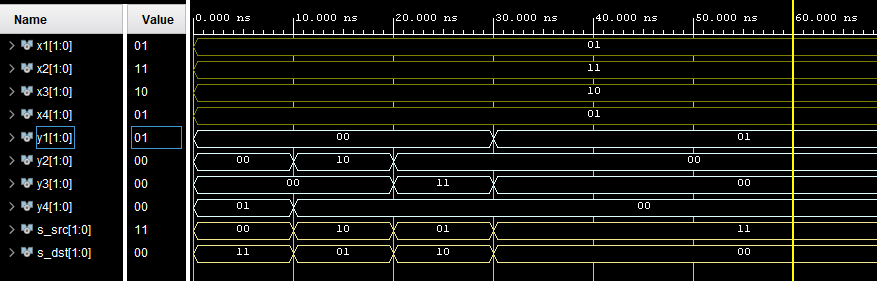
\includegraphics[width=0.95\linewidth]{figure/esercizio11-1/simulazione}
  \caption{Simulazione della omega network a 4 nodi}
  \label{fig:esercizio11-1:simulazione}
\end{figure}

Gli ingressi restano costanti per tutta la durata, mentre \texttt{s\_src} e \texttt{s\_dst} cambiano ogni \SI{10}{\nano\second}. Si legga il secondo intervallo, da \SI{10}{\nano\second} a \SI{20}{\nano\second}: \texttt{s\_src} vale \texttt{"10"} e \texttt{s\_dst} vale \texttt{"01"}, ossia il nodo 3 trasmette al nodo 2. Il dato di \texttt{x3}, \texttt{"10"}, compare su \texttt{y2}, mentre \texttt{y1}, \texttt{y3} e \texttt{y4} restano a \texttt{"00"}. Nello stesso modo, nel primo intervallo \texttt{y4} vale \texttt{"01"}, il valore di \texttt{x1}; nel terzo \texttt{y3} vale \texttt{"11"}, il valore di \texttt{x2}; dal quarto in poi \texttt{y1} vale \texttt{"01"}, il valore di \texttt{x4}.

\begin{risultato}
I quattro trasferimenti producono \texttt{y4} $=$ \texttt{"01"}, \texttt{y2} $=$ \texttt{"10"}, \texttt{y3} $=$ \texttt{"11"} e \texttt{y1} $=$ \texttt{"01"}, e tutte le altre uscite restano a \texttt{"00"}.
\end{risultato}
